\chapter{Umsetzung eines Testprojekts mit Rayden}
\label{cha:Testen}

In diesem Kapitel wird ein Testprojekt mit dem Rayden-System umgesetzt. Dabei wird gezeigt, wie man unterschiedliche Testmethoden mit dem Rayden-System verwenden kann. Um sinnvolle Tests schreiben zu können, wird eine Beispielanwendung benötigt, welche in Abschnitt \ref{cha:demoapp} kurz beschrieben wird. In den nächsten drei Abschnitten \ref{cha:TestenUnit}, \ref{cha:TestenApi} und \ref{cha:TestenUA} wird die Umsetzung von unterschiedlichen Testmethoden mit dem Rayden-System gezeigt. Ein besonderes Augenmerk wird dabei auf die Abnahmetests gelegt.

%%------------------------------------------------------------------------------------------------------

\section{Beispielanwendung \enword{PetClinic}}
\label{cha:demoapp}

Für die Evaluierung des Rayden-Systems wird eine Anwendung zum Testen benötigt. Bei der Anwendung sollte es sich um eine Web-Anwendung handeln, um die Unterstützung von Selenium zeigen zu können. Für die Evaluierung von Rayden wird die \enword{PetClinic}-Web-Anwendung verwendet, welche eine Beispielanwendung des Spring-Projekts ist. Die Abbildung \ref{fig:petClinicPage} zeigt die Startseite dieser Web-Anwendung. Die \enword{PetClinic} mit allen Ressourcen ist öffentlich auf Github unter der Adresse \enword{https://github.com/spring-projects/spring-petclinic/} zugänglich.

\begin{figure}
\centering
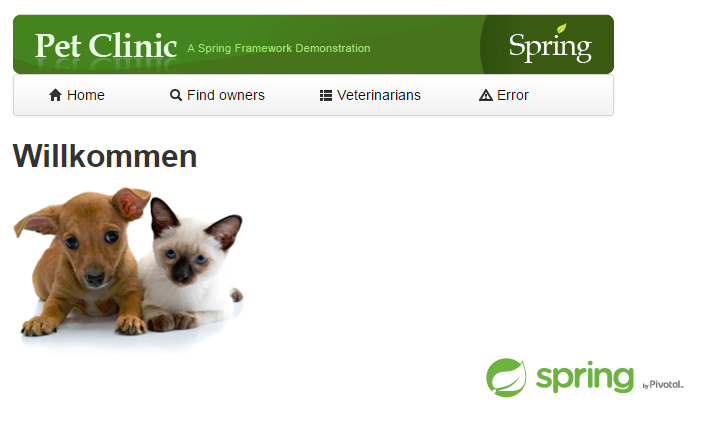
\includegraphics[width=0.9\textwidth]{petclinic.png}
\caption{Startseite der Web-Anwendung \enword{PetClinic}}
\label{fig:petClinicPage}
\end{figure}

\SuperPar
Bei der \enword{PetClinic}-Anwendung handelt es sich um eine Verwaltungssoftware für eine Tierklinik. Mit \enword{PetClinic} können Besuche bei einer Tierärztin oder einem Tierarzt protokolliert werden. Dazu gehört die Erfassung der Tierbesitzerinnen und -besitzer mit ihren Haustieren. Zu jedem Haustier werden alle Arztbesuche gespeichert, damit der Krankheitsverlauf dokumentiert ist. Neben den Besitzerinnen und Besitzern mit ihren Tieren werden zusätzlich Tierärztinnen und -ärzte verwaltet. 

\SuperPar
Da der Funktionsumfang von \enword{PetClinic} überschaubar ist, eignet sich diese ausgezeichnet als Beispielanwendung für die Evaluierung des Rayden-Systems. In den folgenden Abschnitten \ref{cha:TestenUnit}, \ref{cha:TestenApi} und \ref{cha:TestenUA} werden Tests für die \enword{PetClinic}-Anwendung vorgestellt. Diese Tests wurden mit drei unterschiedlichen Testmethoden umgesetzt, um zu zeigen, wie man die Testmethoden mit dem Rayden-System vereinen kann.

%%------------------------------------------------------------------------------------------------------
\section{Komponententest}
\label{cha:TestenUnit}

Dieser Abschnitt zeigt die Umsetzung eines Komponententests mit dem Rayden-System. Für einen Komponententest wird in Rayden zuerst ein \enword{Keyword} angelegt. Der Codeauszug \ref{prog:unitTest} zeigt die Definition dieses \enword{Keywords}. Ein Komponententest wird normalerweise als \enword{Scripted Keyword} umgesetzt und mit dem \enword{Keyword}-Art \enword{unittest} gekennzeichnet. In diesem Beispiel wird die Komponente \enword{PetTypeFormatter} getestet. Diese Komponente der \enword{PetClinic} ist dafür verantwortlich, für eine Zeichenkette das dazugehörige Domänenobjekt zu liefern und umgekehrt. 

\begin{program}
\begin{JavaCode}
unittest Test PetTypeFormatter {
	''' This unittest verifies the functionality of the 
	    formatter class PetTypeFormatter '''
	implemented in java -> "petclinic.TestPetTypeFormatterKeyword"
}
\end{JavaCode}
\caption{Komponententest \enword{Test PetTypeFormatter}}
\label{prog:unitTest}
\end{program}

\SuperPar
Der Codeausschnitt \ref{prog:unitTestImpl} zeigt die Implementierung des \enword{Scripted Keywords}. Die Implementierung des Komponententests ist grundlegend gleich mit einem \enword{JUnit}-Test. Die wesentlichen Unterschiede sind, dass die Methoden nicht mit \enword{@Test} annotiert werden und dass es nur eine Testmethode pro Klasse geben kann. 

\begin{program}
\begin{JavaCode}
public class TestPetTypeFormatterKeyword implements ScriptedKeyword {

  @Override
  public KeywordResult execute(String keyword, KeywordScope scope, 
	  RaydenReporter reporter) throws  AssertionError {
    ClinicService service = new MockClinicService();
    PetTypeFormatter formatter = new PetTypeFormatter(service);

    try {
     Assert.assertEquals("dog", formatter.parse("dog", null).getName());
     Assert.assertEquals("cat", formatter.parse("cat", null).getName());
     Assert.assertEquals("fish",formatter.parse("fish",null).getName());
    } catch (ParseException e) {
      throw new AssertionError(e);
    }
    
    try {
      formatter.parse("hamster", null);
      Assert.fail("No ParseExeption was thrown!");
    } catch (ParseException e) {
    }

    try {
      formatter.parse(null, null);
      Assert.fail("No ParseExeption was thrown!");
    } catch (ParseException e) {
    }

    return new KeywordResult(true);
  } //execute
	
} //TestPetTypeFormatterKeyword
\end{JavaCode}
\caption{Implementierung des \enword{Test PetTypeFormatter} \enword{Keywords}}
\label{prog:unitTestImpl}
\end{program}

\SuperPar
Eine nützliche Erweiterung des Rayden-Systems in der Zukunft wäre zum Beispiel eine bessere Integration mit \enword{Unittest-Frameworks} wie \enword{JUnit} oder \enword{TestNG}.

%%------------------------------------------------------------------------------------------------------
\section{Schnittstellentest}
\label{cha:TestenApi}

Bei einem Schnittstellentest werden öffentliche Schnittstellen, wie eine \enword{RESTful}-Schnittstelle \cite{Rest}, getestet. Der Codeausschnitt \ref{prog:integrationTest} zeigt einen Test, welcher alle Tierärztinnen und -ärzte über eine \enword{RESTful}-Schnittstelle abfragt. Schnittstellentests können entweder als \enword{Compound Keywords} oder als \enword{Scripted Keywords} definiert werden. Es hängt ganz davon ab, ob die Implementierung des \enword{Scripted Keywords} in einem anderen Test wieder verwendet werden kann. 

\begin{program}
\begin{JavaCode}
apitest Test Veterinarians RESTful Service {
	'''This keyword checks the restful service for veterinarians.'''
	
	Verify JSON("http://localhost:9966/petclinic/vets.json", 
	            "./demodata/vets.json")
}

keyword Verify JSON {
  '''The keyword downloads the content from the given url. A second 
	   content is loaded from the file. The both contents are parsed
		 into a JSON object tree. If the two trees are equal, the 
		 keyword finishes successfully'''
		
	parameter url
	parameter file

	implemented in java -> "petclinic.VerifyJsonKeyword"
}
\end{JavaCode}
\caption{Integrationstest \enword{Test Veterinarians RESTful Service}}
\label{prog:integrationTest}
\end{program}

\SuperPar 
Bei diesem Beispiel liefert die Schnittstelle das Ergebnis als \enword{JSON}-Text (\enword{JavaScript Object Notation}). Bei \enword{JSON} handelt es sich um ein Datenformat, bei dem die Daten in Attribute-Wert-Paaren angeordnet werden.  Um zu überprüfen, ob die Schnittstelle korrekt funktioniert, wird dieser Text mit einem Text aus einer Demodaten-Datei verglichen. Damit der Test erfolgreich durchläuft, müssen die beiden Texte semantisch gleich sein. Zwei \enword{JSON}-Texte sind semantisch gleich, wenn die beiden Objektgraphen gleich sind. Die serialisierte Form ist dafür aber nicht entscheidend.

\begin{program}
\begin{JavaCode}
public class VerifyJsonKeyword implements ScriptedKeyword {

  @Override
  public KeywordResult execute(String keyword, KeywordScope scope, 
	  RaydenReporter reporter) throws RuntimeException {
    String url = scope.getVariableAsString("url");
    String file = scope.getVariableAsString("file");

    try {
      CloseableHttpClient client = HttpClientBuilder.create().build();
      CloseableHttpResponse response = client.execute(new HttpGet(url));
      if (response.getStatusLine().getStatusCode() != 200) {
        return new KeywordResult(false);
      }
      String json = IOUtils.toString(response.getEntity().getContent());

      JsonParser parser = new JsonParser();
      JsonElement o1 = parser.parse(json);
      JsonElement o2 = parser.parse(IOUtils.toString(
			  new FileInputStream(file)));

      return new KeywordResult(o1.equals(o2));
    } catch (IOException e) {
      throw new RuntimeException(e);
    }
  } //execute
	
} //VerifyJsonKeyword
\end{JavaCode}
\caption{Implementierung des \enword{Verify Json Keywords}}
\label{prog:integrationTestImpl}
\end{program}

\SuperPar
Wenn mehrere Schnittstellen dieser Art getestet werden, ist es sinnvoll, dass man die Funktionalität zum Abfragen und Vergleichen der Daten in ein separates \enword{Keyword} kapselt. Dadurch können andere Tests dieses \enword{Keyword} wiederverwenden. Das Codebeispiel \ref{prog:integrationTestImpl} zeigt die Implementierung des \enword{Verify Json Keywords}. Am Beginn des Codestücks wird zuerst über einen \enword{HttpClient} der \enword{JSON}-Text von einem Server abgefragt. Danach wird der \enword{JSON}-Text mit einem \enword{Parser} in einen Objektgraph transformiert. Dafür wird eine \enword{Parser}-Implementierung aus der \enword{Google-Guava}-Bibliothek \cite{Guava} verwendet. Derselbe Prozess wird auch mit der Demodaten-Datei durchlaufen. Am Ende gibt es zwei Objektgraphen für die \enword{JSON}-Texte. Für den semantischen Vergleich der beiden Graphen kann die Methode \enword{equals()} der Klasse \enword{JsonElement} verwendet werden. Diese Klasse stammt wiederum aus der \enword{Google-Guava}-Bibliothek.

%%------------------------------------------------------------------------------------------------------
\section{Abnahmetests}
\label{cha:TestenUA}

In diesem Abschnitt wird die letzte Testmethode für die Evaluierung erläutert. Dabei handelt es sich um den Abnahmetest, die wohl wichtigste Testmethode für das Rayden-System. Ein Großteil des Rayden-Systems ist primär für die Unterstützung dieser Testmethode entwickelt worden. Aus diesem Grund enthält dieser Abschnitt auch zwei Umsetzungen von Testmethoden mit Rayden. Als erstes wird der Testfall \enword{Find a pet owner and check the details} \ref{cha:TestenUA1} umgesetzt. Bei diesem Testfall wird die Suche der \enword{PetClinic}-Anwendung getestet. Im zweiten Testfall \ref{cha:TestenUA2} wird das Anlegen einer neuen Tierbesitzerin oder eines neuen Tierbesitzers gezeigt. 

\SuperPar
Für das Steuern der Browser wurde für beide Abnahmetests die Selenium-Bibliothek verwendet. Aus diesem Grund wird im dritten Teil \ref{cha:TestenSelenium} dieses Abschnittes die Bindung zwischen dem Rayden-System und der Selenium-Bibliothek gezeigt. 

%%------------------------------------------------------------------------------------------------------

\subsection{Abnahmetest \enword{Find a pet owner and check the details}}
\label{cha:TestenUA1}

Bei dem  Abnahmetest im Codeausschnitt \ref{prog:uatest-find} wird die Suchfunktion der \enword{PetClinic}-Anwendung getestet. Dafür wird der Testfall zu erst in die zwei \enword{Compound Keywords} \enword{Find a specific Pet Owner} und \enword{Check Owner Details} aufgeteilt. Neben den beiden \enword{Keywords} werden noch die zwei weiteren \enword{Keywords} \enword{Prepare Browser} und \enword{Cleanup Browser}  benötigt, welche für das Starten und Stoppen des Browsers zuständig sind. 

\begin{program}
\lstinputlisting{samplecode/uatest-findpetowner.rlg}
\caption{Abnahmetest \enword{Find a pet owner and check the details}}
\label{prog:uatest-find}
\end{program}


\begin{program}
\lstinputlisting{samplecode/or-findpetowner.rlg}
\caption{Codeauszug aus dem \enword{Object Repository} für den Testfall \enword{Find a pet owner and check the details}}
\label{prog:or-find}
\end{program}

\SuperPar
Das \enword{Keyword} \enword{Find a specific Pet Owner} führt die Suche nach einer Tierbesitzerin mit dem Namen \enword{Davis} aus. Dafür navigiert das \enword{Keyword} auf die Seite für Tierbesitzerinnen und Tierbesitzer und startet die Suche. Danach werden auf der Ergebnisseite der Suche alle Besitzerinnen und Besizter aufgelistet, welche in der Anwendung vorhanden sind. Danach wird mithilfe der integrierten Suche nach dem Namen \enword{Davis} gesucht und die Detailseite der Tierbesitzerin geöffnet. Wurde die Detailseite erfolgreich geöffnet, ist das \enword{Keyword} fertig abgearbeitet. Die Validierung der Daten wird von dem nächsten \enword{Keyword} \enword{Check Owner Details} durchgeführt.

\SuperPar
Dem \enword{Keyword} \enword{Check Owner Details} werden die zu überprüfenden Daten als Parameter übergeben. Das \enword{Keyword} überprüft jedes Datum mit dem \enword{Scripted Keyword} \enword{Verify Text}. Dem \enword{Scripted Keyword} werden zwei Parameter übergeben. Der erste Parameter ist ein \enword{Locator}, welcher ein Element auf der Web-Seite definiert. Von diesem Element wird der Text abgefragt und mit dem zweiten Parameter verglichen. Der zweite Parameter ist eine Zeichenkette mit dem erwarteten Wert. Sind die Werte nicht gleich, wird der Test mit einem Fehler abgebrochen. 

\begin{figure}
\centering
\includegraphics[width=1\textwidth]{or.png}
\caption{Darstellung der Verbindung eines Objekts aus dem \enword{Object Repository} mit Elementen auf der Web-Seite}
\label{fig:orwebsite}
\end{figure}

\SuperPar
Damit in den \enword{Keywords} keine \enword{XPath}-Ausdrücke vorkommen müssen, wird ein \enword{Object Repository} verwendet. Einen Auszug mit den wichtigsten Objekten für diesen Abnahmetest zeigt das Codebeispiel \ref{prog:or-find}. Dieses Codebeispiel enthält die Objekte für die Suchergebnisseite und die Detailseite für Tierbesitzerinnen und Tierbesitzer. Die Abbildung \ref{fig:orwebsite} zeigt die Verbindung von Web-Seiten-Elementen auf Objekte im \enword{Object Repository}. In der Grafik sind jene Elemente rot hinterlegt, welche einen Eintrag im \enword{Object Repository} besitzen. Neben jedem Element steht auch der vollständige \enword{Locator}, mit welchem man das Objekt aus \enword{Object Repository} abfragen kann.

%%------------------------------------------------------------------------------------------------------

\subsection{Abnahmetest \enword{Add new pet owner}}
\label{cha:TestenUA2}


Der zweite Abnahmetest testet den Anwendungsfall \enword{Add new pet owner}. Dieser Abnahmetest wird direkt im Abnahmetest-\enword{Keyword} spezifiziert. Zuerst wird wieder die Testumgebung mit dem \enword{Keyword} \enword{Prepare Browser} vorbereitet. Im nächsten Schritt navigiert der Test auf die Tierbesitzerinnen- und Tierbesitzerseite und betätigt auf die Schaltfläche \enword{Add Owner}. 


\SuperPar
Danach werden alle benötigten Daten für eine neue Tierbesitzerin oder einen neuen Tierbesitzer im Formular eingegeben. Dazu wird das \enword{Keyword} \enword{Type Text} verwendet. Dieses \enword{Scripted Keyword} schreibt mithilfe der Selenium-Bibliothek einen Text in ein Textfeld auf der Web-Seite. Der Codeauszug \ref{prog:or-create} zeigt die dazugehörigen Objekte im \enword{Object Repository}. Der Auszug zeigt die Seite \enword{Edit Owner Page}, welche das Formular für das Anlegen und Ändern einer Besitzerin oder eines Besitzers zeigt.

\SuperPar
Das \enword{Add new pet owner} \enword{Keyword} ist ein gutes Beispiel, um zu zeigen, wie man mithilfe des \enword{Object Repositories} einen leserlichen Test schreiben kann. Der Test setzt ausschließlich auf \enword{Locators}  und verzichtet auf die direkte Verwendung von \enword{XPath}-Ausdrücken. 

\begin{program}
\lstinputlisting{samplecode/or-createpetowner.rlg}
\caption{Codeauszug aus dem \enword{Object Repository} für den Testfall \enword{Add new pet owner}}
\label{prog:or-create}
\end{program}

%%------------------------------------------------------------------------------------------------------

\subsection{\enword{Keywords} aus der Selenium-Bibliothek}
\label{cha:TestenSelenium}

In diesem Abschnitt werden ausgewählte Selenium-\enword{Keywords} aus den Abnahmetests beschrieben. Diese \enword{Keywords} wurden alle in der Datei \enword{selenium.rlg} angelegt. Die Datei \enword{selenium.rlg} stellt somit die \enword{Bridge} zwischen Rayden und Selenium dar. Das Codestück \ref{prog:selenium} zeigt drei \enword{Scripted Keywords}, welche einen guten Überblick in die Integration von Selenium in das Rayden-System zeigen. 

\begin{program}
\lstinputlisting{samplecode/selenium.rlg}
\caption{Codeauszug aus der Selenium-\enword{Keyword}-Bibliothek}
\label{prog:selenium}
\end{program}

\SuperPar
Zuerst wird im Codeausschnitt \ref{prog:openBrowserKeyword} das \enword{Open Browser Keyword} beschrieben. Dieses \enword{Scripted Keyword} ist essentiell für die Verwendung von Selenium, da dieses \enword{Keyword} die Testumgebung vorbereitet. Als Parameter werden der Browsertyp und eine \enword{URL} übergeben. Der Browsertyp definiert den Browser, welcher gestartet werden soll. Das kann zum Beispiel der \enword{Internet Explorer}, \enword{Firefox} oder \enword{Google Chrome} sein. Mit dem Browsertyp-Parameter wird ein \enword{Webdriver}-Objekt angelegt. Dieses Objekt dient als Schnittstelle zwischen dem Test und der Browser-Instanz. Jedes neue \enword{Webdriver}-Objekt startet einen Browser. Der zweite Parameter \enword{URL} definiert die Startseite. Über die Methode \enword{navigate()} der Klasse \enword{Webdriver} kann man auf eine neue Seite im Browser navigieren. 

\begin{program}
\begin{JavaCode}
public class OpenBrowserKeyword implements ScriptedKeyword {

	@Override
	public KeywordResult execute(String keyword, KeywordScope scope, 
	  RaydenReporter reporter) {
		String browserType = scope.getVariableAsString("browserType");
		String url = scope.getVariableAsString("url");
		WebDriver driver = Selenium.getInstance()
		  .initializeDriver(browserType);
		driver.navigate().to(url);
		return new KeywordResult(true);
	} //execute
	
} //OpenBrowserKeyword
\end{JavaCode}
\caption{Implementierung des \enword{Open Browser Keywords}}
\label{prog:openBrowserKeyword}
\end{program}

\SuperPar
Bei dem nächsten \enword{Keyword} handelt es sich um das \enword{Click Keyword}, welches im Codestück \ref{prog:clickKeyword} gezeigt wird. Mit diesem \enword{Keyword} kann man einen Klick auf der Web-Seite simulieren. Um die richtige Position für den Mauszeiger herausfinden zu können, wird dem \enword{Keyword} ein \enword{Locator} übergeben. Dieser \enword{Locator} beschreibt ein Element auf der Web-Seite. Die Auswertung dieses \enword{Locators} wird von der Methode \enword{findElement()} übernommen. Die Methode greift auf das aktuelle \enword{WebDriver}-Objekt zu, um das Element zu finden. Diese Aktion könnte man auch direkt über das \enword{WebDriver}-Objekt ausführen, jedoch enthält die Methode \enword{findElement()} aus der Selenium-Klasse eine zusätzliche Wiederholungsfunktion im Fall eines Fehlers. Die Funktionalität ist für einen stabilen Abnahmetest wichtig, da diese Synchronisierungsprobleme mit der Web-Anwendung reduziert. 

\begin{program}
\begin{JavaCode}
public class ClickKeyword implements ScriptedKeyword {

  @Override
  public KeywordResult execute(String keyword, KeywordScope scope, 
	  RaydenReporter reporter) {
    RaydenExpressionLocator locator = 
		  (RaydenExpressionLocator) scope.getVariable("locator");
    reporter.log("Click on '" + locator + "'");
    Selenium.getInstance().findElement(locator.getEvalLocator())
		  .click();
    return new KeywordResult(true);
  } //execute
	
} //ClickKeyword
\end{JavaCode}
\caption{Implementierung des \enword{Click Keywords}}
\label{prog:clickKeyword}
\end{program}

\SuperPar
Man spricht von einem Synchronisierungsfehler bei einer Web-Seite, wenn eine Aktion ausgeführt wird, obwohl die Anwendung noch nicht fertig geladen wurde. Dieser Fehler tritt häufig bei stark dynamischen Web-Seiten auf. Die einfachste Lösung für das Problem ist die mehrmalige Auswertung des \enword{XPath}-Ausdrucks, falls dieser kein Element findet. Genau dieser Ansatz ist auch in der \enword{findElement()}-Methode der Selenium-Klasse implementiert.

\begin{program}
\begin{JavaCode}
public class VerifyTextKeyword implements ScriptedKeyword {

  @Override
  public KeywordResult execute(String keyword, KeywordScope scope,
	  RaydenReporter reporter) {
    RaydenExpressionLocator locator = 
		  (RaydenExpressionLocator) scope.getVariable("locator");
    String text = scope.getVariableAsString("text");
    WebElement element = Selenium.getInstance().findElement(
		  locator.getEvalLocator());
    String elementText = element.getText();
    reporter.log("Verify Text: '" + text + "'='" + elementText + "'");
    return new KeywordResult(text.equals(elementText));
  } //execute
	
} //VerifyTextKeyword
\end{JavaCode}
\caption{Implementierung des \enword{Verify Text Keywords}}
\label{prog:verifyTextKeyword}
\end{program}

\SuperPar
Bei dem \enword{Keyword} \enword{Verify Text} handelt es sich um eine Überprüfung. Mit diesem \enword{Keyword} kann ein Text auf einer Web-Seite mit einem vordefinierten Text verglichen werden. Bei einem Fehlerfall wird das \enword{Keyword} mit einem Fehler beendet und die Ausführung des Tests abgebrochen. Die Implementierung des \enword{Scripted Keywords} zeigt der Codeausschnitt \ref{prog:verifyTextKeyword}. Das Ergebnis des Vergleichs der beiden Texte wird an ein \enword{KeywordResult}-Objekt übergeben. 

\SuperPar
Dieses Kapitel hat gezeigt, wie man ein Testprojekt mit Rayden umsetzen kann. Dafür wurden drei unterschiedliche Testmethoden gezeigt und erläutert, wie diese mit Rayden umgesetzt werden können. Die Testbeispiele haben auch gezeigt, welche Vorteile die Verwendung des \enword{Object Repositories} hat. Das nächste Kapitel bietet eine Zusammenfassung dieser Masterarbeit und gibt einen Ausblick auf mögliche Erweiterungen des Rayden-Systems. 